\section{Polynomial}
We include this test case because of the analytic solution, mean, and variance.  

\subsection{Univariate}
The test code simply solves the function evaluation
\begin{equation}
U(\theta) = 1+2\theta.
\end{equation}
To find the first and second moments of the function $U(\theta)$ analytically,
\begin{align}
\expv{U(\theta)}=\expv{1+2\theta}&=1+2\expv{\theta},\\
\expv{U(\theta)^2}\expv{(1+2\theta)^2}&=1+4\expv{\theta}+4\expv{\theta^2}.
\end{align}
In general, the moments of $\theta$ are given as
\begin{equation}
m_r(\theta)=\expv{\theta^r}=\int_\Omega P(\theta)\theta^r d\theta.
\end{equation}

We consider the cases when $\theta$ has a uniform distribution $\theta\in[3,7]$ as well as a normal distribution $\theta\in\mathcal{N}(5,4)$.  When using PCESC, all coefficients for expansions of polynomial order higher than 1 are zero; thus, only the results for order 2 expansion are shown.

\subsubsection{Uniform Distribution}
For a uniformly-distributed variable $\xi\in[a,b]$, the moments are given as
\begin{equation}
m_r(\xi)=\int_{a^r}^{b^r} \frac{1}{b^r-a^r}\xi^r d\xi.
\end{equation}
Of particular interest are the first moment (expected value) and second moment, which we use to calculate variance.
\begin{align}\label{eq:anl moments uni}
m_1(\xi)\equiv\expv{\xi}&=\frac{a+b}{2},\\
m_2(\xi)=\expv{\xi^2}&=\frac{1}{3}(b^2+ab+a^2).
\end{align}
Using the analytic moments given in Eq. \ref{eq:anl moments uni},
\begin{align}
\expv{\theta} &= 5,\\
\expv{\theta^2}&=\frac{79}{3},\\
\expv{U(\theta)}&=11,\\
\expv{U(\theta)^2}&=\frac{379}{3}.
\end{align}
The variance is given simply as
\begin{equation}
\text{var}[U(\theta)]=\expv{U(\theta)^2}-\expv{U(\theta)}^2=\frac{79}{3}.
\end{equation}
The statistics from MC and PCESC are given in Table \ref{tab:poly uniform} and the pdfs are in Fig. \ref{fig:poly uni}.


\begin{table}[H]
\begin{center}
\begin{tabular}{c c|l l}
type & runs/order & mean & variance \\ \hline
Analytic & - & 11 & 16/3 \\
MC & $1\times10^7$ & 10.999555712 & 5.3374535046 \\
SC & 2 & 11.0 & 5.33333333333 \\
\end{tabular}
\end{center}
\caption{Polynomial Test, Monovariate Uniform Distribution Statistics}
\label{tab:poly uniform}
\end{table}

\begin{figure}[H]
\centering
%  \begin{subfigure}[b]{0.45 \textwidth}
   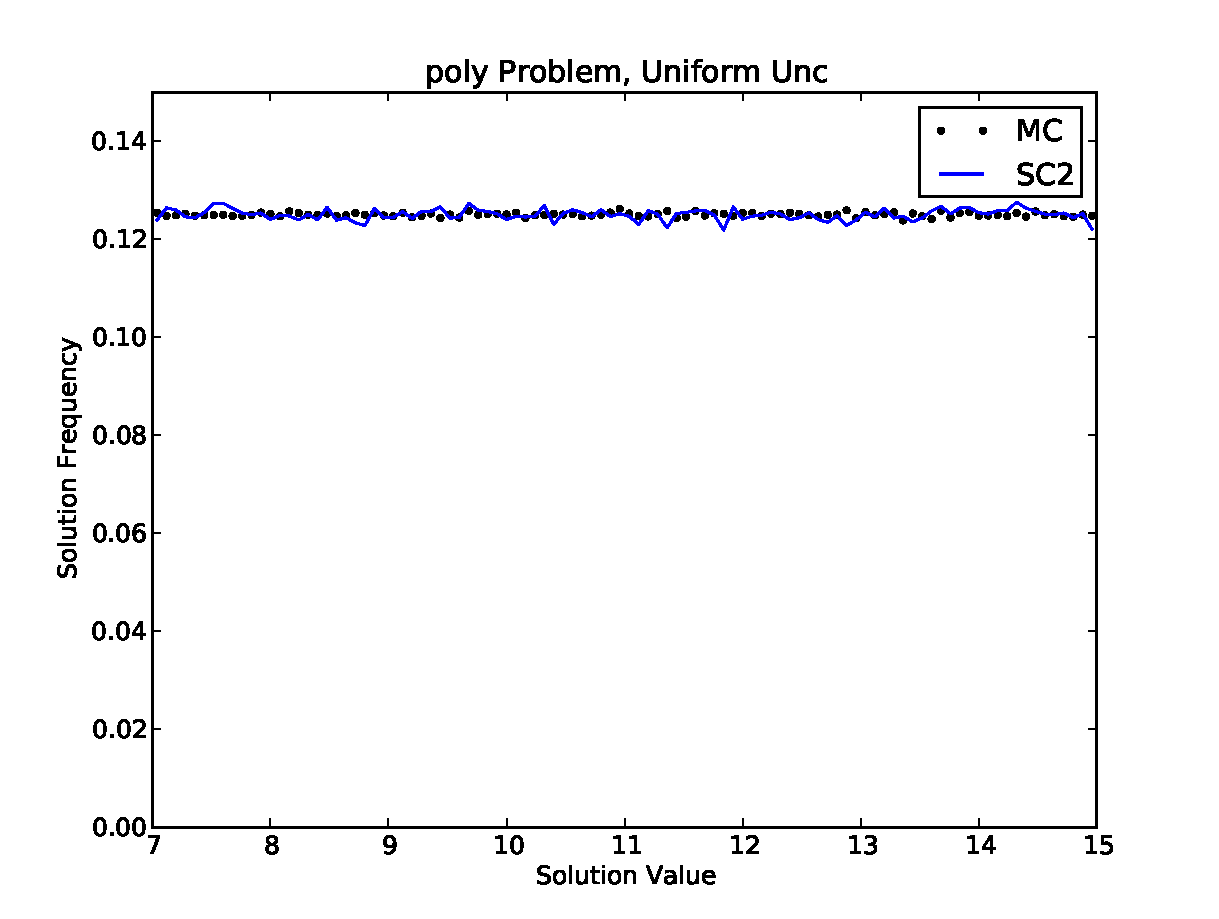
\includegraphics[width=0.7\textwidth]{../graphics/poly_uniform_pdfs}
   \caption{Polynomial Problem, Uniform PDFs}
      \label{fig:poly uni}
%  \end{subfigure}
\end{figure}

\subsubsection{Normal Distribution}
For a normally-distributed variable $\xi\in[\mu,\sigma^2]$, the moments are given as
\begin{equation}
m_r(\xi)=\int_{-\infty}^\infty \frac{1}{\sqrt{2\pi\sigma^2}}e^{-\frac{(x-\mu)^2}{2\sigma^2}}\xi^r d\xi.
\end{equation}
The analytic statistical measures of interest are
\begin{align}\label{eq:anl moments norm}
m_1(\xi)\equiv\expv{\xi}&=\mu,\\
m_2(\xi)=\expv{\xi^2}&=\mu^2+\sigma^2.
\end{align}
Using the analytic moments given in Eq. \ref{eq:anl moments norm},
\begin{align}
\expv{\theta} = 5, &\hspace{30pt}\expv{\theta^2}=29,\\
\expv{U(\theta)}=11, &\hspace{30pt}\expv{U(\theta)^2}=137.
\end{align}
The variance is given simply as
\begin{equation}
\text{var}[U(\theta)]=\expv{U(\theta)^2}-\expv{U(\theta)}^2=16.
\end{equation}
The statistics from MC and PCESC are given in Table \ref{tab:poly normal} and the pdfs are in Fig. \ref{fig:poly norm}.

\begin{table}[H]
\begin{center}
\begin{tabular}{c c|l l}
type & runs/order & mean & variance \\ \hline
Analytic & - & 11 & 16 \\
MC & $1\times10^7$ & 11.0000448162 & 15.9892244775 \\
SC & 2 & 11 & 16 \\
\end{tabular}
\end{center}
\caption{Polynomial Test, Monovariate Normal Distribution Statistics}
\label{tab:poly normal}
\end{table}

\begin{figure}[H]
\centering
%  \begin{subfigure}[b]{0.45\textwidth}
   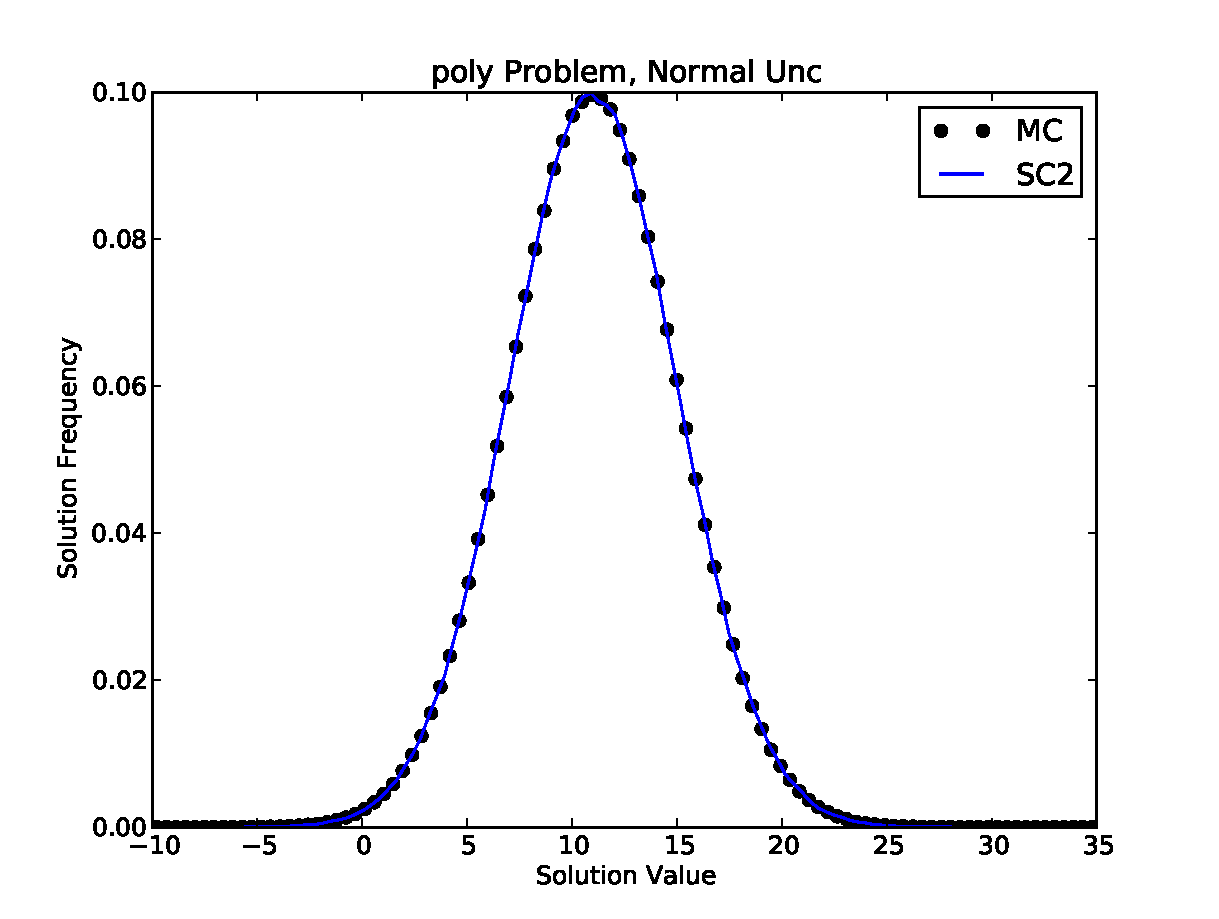
\includegraphics[width=0.7\textwidth]{../graphics/poly_normal_pdfs}
   \caption{Polynomial Problem, Normal PDFs}
      \label{fig:poly norm}
%  \end{subfigure}
%\caption{Polynomial Problem Solution Distributions}
%\label{fig:polypdfs}
\end{figure}



\subsection{Bivariate}
Similar to the univariate case, we add a dimension and define a new function to sample
\begin{equation}
U(\vb*{\theta})=U(\theta_1,\theta_2)=\theta_1\qty(1+\theta_2).
\end{equation}
We impose independence between the uncertain variables in $\vb*{\theta}$.
The expected value is given as
\begin{align}
\ev{U}&=\ev{\theta_1}+\ev{\theta_1\theta_2},\\
  &= \ev{\theta_1}\qty(1+\ev{\theta_2}).
\end{align}
The second moment is
\begin{align}
\ev{U^2}=\ev{\theta_1^2}\qty(1+2\ev{\theta_2}+\ev{\theta_2^2}).
\end{align}

\subsubsection{Uniform}
We allow $\vb*{\theta}$ to vary uniformly as
\begin{align}
\theta_1 &\in[3,7],\\
\theta_2 &\in[1,6].
\end{align}
Using the derivations for the univariate uniform variable, moments are given explicitly by
\begin{align}
\ev{U}&=(5)+(5)\qty(\frac{7}{2}), \\
  &= \frac{45}{2}.\\
\ev{U^2} &= \frac{(3)^2+(3)(7)+(7)^2}{3}\qty(1+(1+6)+\frac{(1)^2+(1)(6)+(6)^2}{3}),\\
  &= 588.\bar1.
\end{align}
The variance is
\begin{equation}
\text{var}[U]=\ev{U^2}-\ev{U}^2=81.86\bar1.
\end{equation}
The analytic, MC, and PCESC statistics are in Table \ref{tab:2v poly uniform}, and the pdfs are show in Fig. \ref{fig:2v poly uni}.

\begin{table}[H]
\begin{center}
\begin{tabular}{c c|l l}
type & runs/order & mean & variance \\ \hline
Analytic & - & $45/2$ & $81.86\bar1$ \\
MC & $1\times10^7$ & 22.4962950638 & 81.8754664265 \\
SC & (1,1) & 22.5 & 81.8611111111 \\
\end{tabular}
\end{center}
\caption{Polynomial Test, Bivariate Uniform Distribution Statistics}
\label{tab:2v poly uniform}
\end{table}

\begin{figure}[H]
\centering
%  \begin{subfigure}[b]{0.45 \textwidth}
   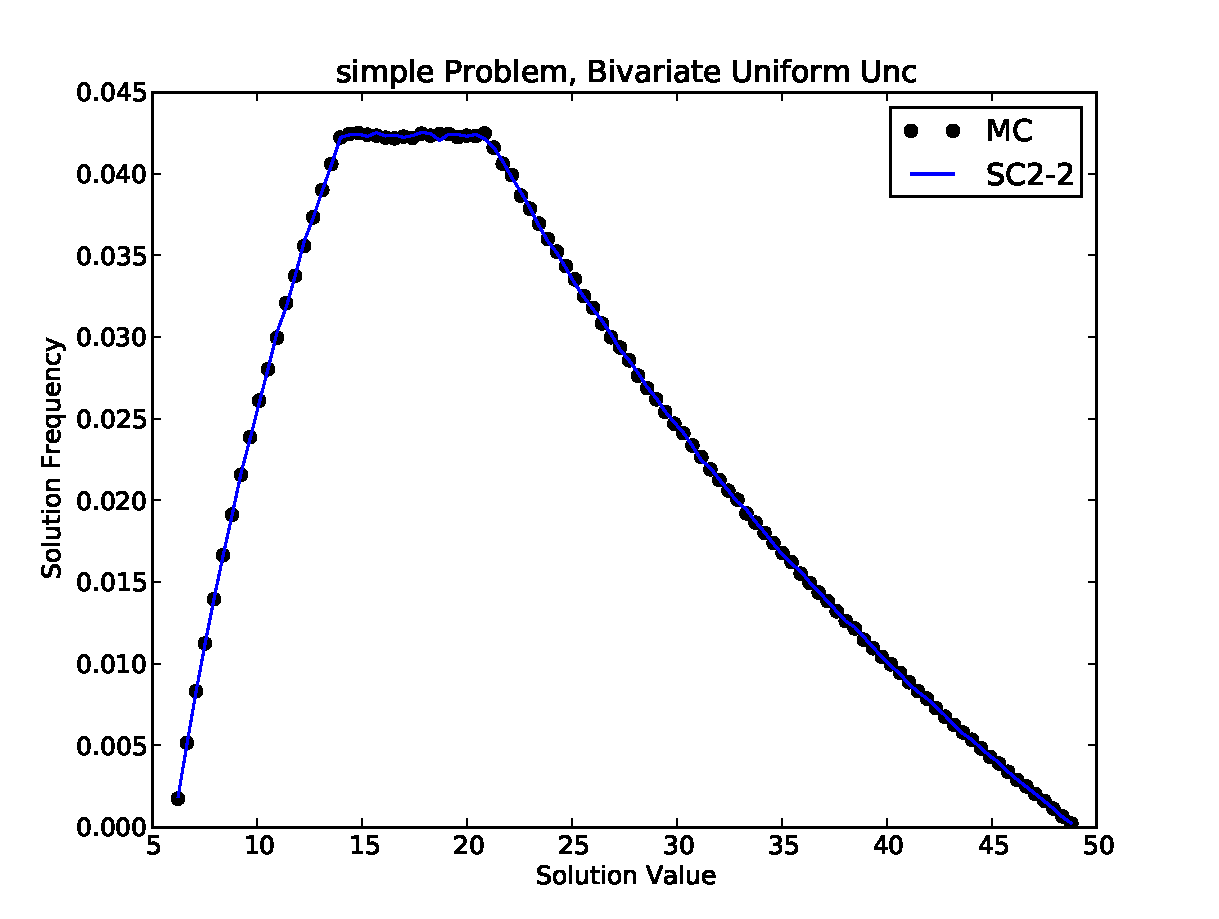
\includegraphics[width=0.7\textwidth]{../graphics/poly_2v_uniform_pdfs}
   \caption{Polynomial Problem, Bivariate Uniform PDFs}
      \label{fig:2v poly uni}
%  \end{subfigure}
\end{figure}